\chapter{The source calibration in water phase}
\label{chap:neutronDet}

\subsection{The calibration information}
Americium-Beryllium~(\ce{AmBe}) and Americium-Carbon~(\ce{AmC}) neutron sources serve as critical reference standards for characterizing neutron detecting capabilities. Both sources leverage the alpha decay of \ce{^241Am}. The neutron producing process can be described as Eq.~\eqref{eq:amn}:
\begin{equation}
	\label{eq:amn}
	{ }_{95}^{241} \mathrm{Am} \rightarrow{ }_{93}^{237} \mathrm{~Np}+{ }_2^4 \mathrm{He} \begin{cases}{ }_4^9 \mathrm{Be}+{ }_2^4 \mathrm{He} \rightarrow{ }_6^{12} \mathrm{C}+{ }_0^1 \mathrm{n} & (4.44 \mathrm{MeV}~\gamma) \\ { }_6^{12} \mathrm{C}+{ }_2^4 \mathrm{He} \rightarrow{ }_7^{15} \mathrm{~N}+{ }_0^1 \mathrm{n} & (6.13 \mathrm{MeV}~\gamma)\end{cases}
\end{equation}

During the water phase, neutron source calibration was performed three times, and the summary of 14 runs are in Table.~\ref{tab:summaryOfRuns}.
\begin{table}[htbp]
	\centering
	\caption{The neutron source calibration in water phase}%标题
	\label{tab:summaryOfRuns}
	\begin{tabular}{ccc}
		\toprule
		\textbf{Calibration} & \textbf{Date} & \textbf{Configuration}                  \\
		\midrule
		First                & 02/02         & \makecell[c]{\ce{AmC}, threshold=53,    \\ Run~3279, 3281, 3283, 3286, 3293}  \\
		Second               & 02/03         & \makecell[c]{\ce{AmBe}, threshold=53,   \\ Run~3333, 3335, 3338, 3340, 3342} \\
		Final                & 02/07         & \makecell[c]{\ce{AmBe}, threshold=46.5, \\Run~3660, 3663, 3671; \\ \ce{AmC}, threshold=44, Run~3675} \\
		\bottomrule
	\end{tabular}
\end{table}
All the calibration sources were placed along the z-axis, as Fig.~\ref{fig:calib_set} shown.
\begin{figure}[htbp]
	\centering
	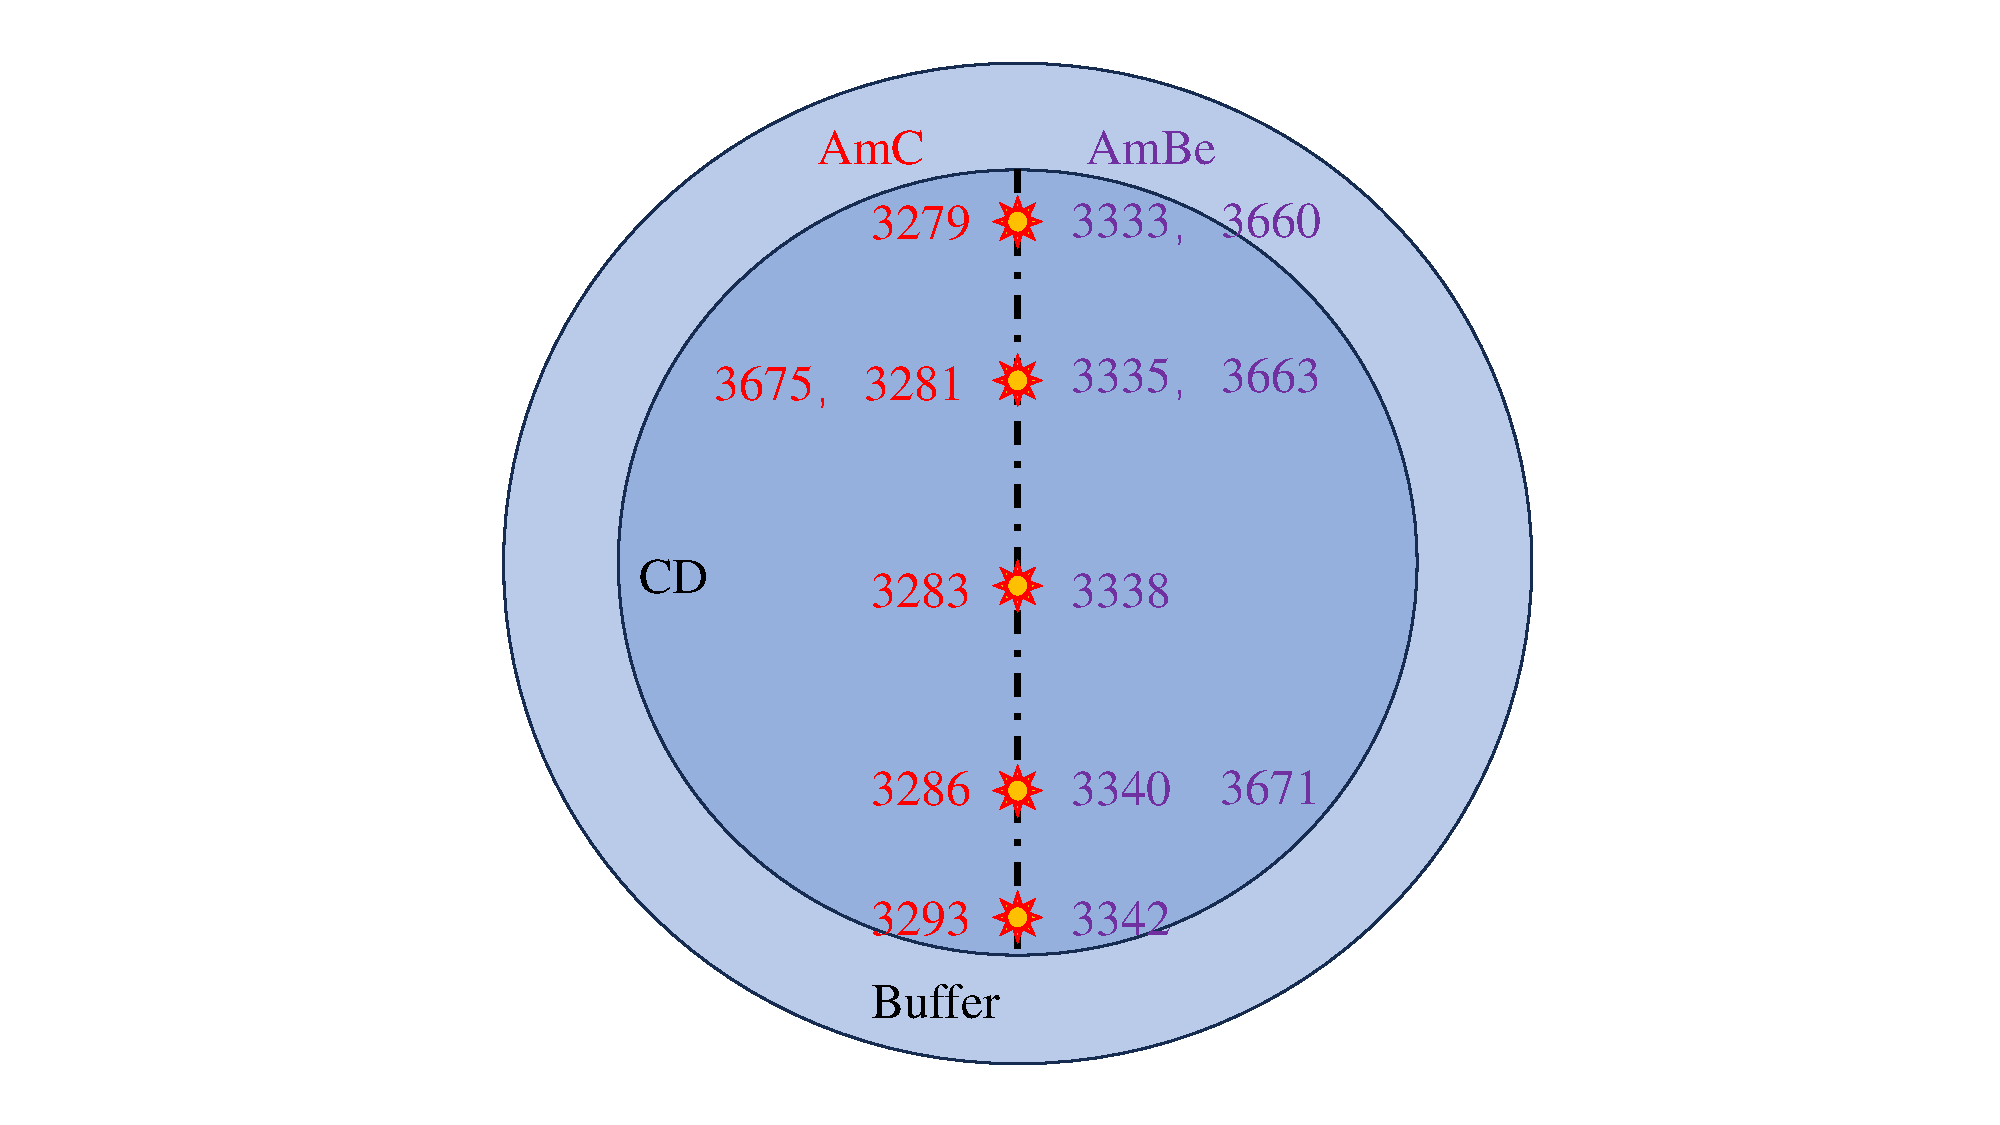
\includegraphics[width=0.5\textwidth]{neutron_calib/calib_set.pdf}
	\caption{The calibration source positions in water phase.}
	\label{fig:calib_set}
\end{figure}
To enhance our capability in studying low-energy events in water phase, we decouple and analyze prompt and delayed signals separately during the calibration source analysis.
\section{JUNO's low-energy threshold in water phase}
\label{sec:lowenergy}
\subsection{The reconstruction of the prompt signals}
\subsubsection{The event selection before reconstruction}
\label{subsec:preselect}
In this study, we take Run~3671~(calibrated with a \ce{AmBe} source at the position of (0, 0, \SI{-10}{m})) as an illustrative example. To mitigate the data volume, we selectively choose a subset of events from the previous findings (JUNO-doc-12539) based on Baona's reconstruction method. Additionally, partial background events are filtered out. After applying a fiducial volume of \SI{17}{m} cut, we observed that a large number of events were downward, as depicted in Fig.~\ref{fig:downwards}.
\begin{figure}[htbp]
	\centering
	\includegraphics[page=9,width=0.45\textwidth]{neutron_calib/selection/3671.pdf}
	\caption{The distribution of $p_z/p$ after applying a fiducial volume of \SI{17}{m} cut.}
	\label{fig:downwards}
\end{figure}

We require additional directional cuts. Therefore, our selection criteria are as follows.
\begin{itemize}
	\item Fiducial volume $r < \SI{17}{m}$
	\item isglass $< 0.5$
	\item score $>0.001$
	\item $p_z/p>-0.8$
	\item $n_{20}>12$
\end{itemize}
To demonstrate the events selection during the cut process, we apply a cylindrical cut with a radius of \SI{2}{m} along the z-axis and plot the z-coordinate distribution of events as shown in Fig.~\ref{fig:selectionFromBaona}.

\begin{figure}[htbp]
	\centering
	\begin{subfigure}{0.5\textwidth}
		\centering
		\includegraphics[page=5,width=0.9\textwidth]{neutron_calib/selection/3671.pdf}
		\label{fig:nocylinder}
		% 图片宽度占子图宽度的80%
	\end{subfigure}% 
	\begin{subfigure}{0.5\textwidth}
		\centering
		\includegraphics[page=3,width=0.9\textwidth]{neutron_calib/selection/3671.pdf}
		\label{fig:cylinder}
	\end{subfigure}
	\caption{The distribution of z-coordinate in Run~3671. \subref{fig:nocylinder} shows the distribution without cylindrical cut, while \subref{fig:cylinder} shows the distribution after the cut.}
	\label{fig:selectionFromBaona}
\end{figure}

After event selection, additional constraints are applied to the PMT photoelectron (PE) timing distribution.
The PE times are binned with a width of \SI{48}{ns} over the interval $t \in [96,576]\si{ns}$.
A \SI{180}{ns} reconstruction window is then defined, comprising \SI{36}{ns} before and \SI{144}{ns} after the maximum bin within the search range, as illustrated in Fig.~\ref{fig:PEtime}.
This selection effectively suppresses dark noise contributions and improves the robustness of the vertex reconstruction.
\begin{figure}[htbp]
	\centering
	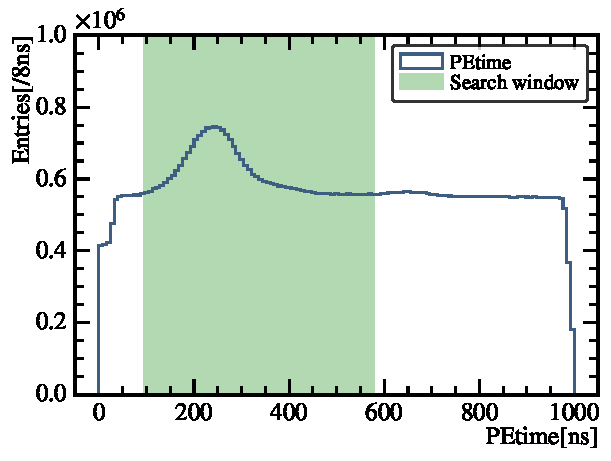
\includegraphics[width=0.5\textwidth]{neutron_calib/PEtime.pdf}
	\caption{The PE time distribution in Run~3671. We search the maximum bin in the green range and select a \SI{180}{ns} time window for reconstruction.}
	\label{fig:PEtime}
\end{figure}

\subsubsection{The position distribution of the prompt signals}
The prompt signal reconstruction employs the maximum likelihood method described in Sec.~\ref{sec:recon}.
Subsequently, quality and background rejection cuts are applied to remove events with poor reconstruction performance and residual background contamination. The specific cuts are as follows:
\begin{itemize}
	\item Fiducial volume: $r<16.5\si{m}$
	\item Unknown downwards events: $p_z/p>-0.8$
	\item Signal quality: $k>-0.85$
	\item Energy related: $n_{10}-n_{b}>15$ and $n_c>8$
\end{itemize}

\begin{figure}[htbp]
	\centering
	\includegraphics[page=9,width=\textwidth]{neutron_calib/prompt/3671.pdf}
	\caption{The position distribution of the prompt signals in Run~3671.}
	\label{fig:positionPrompt}
\end{figure}
After these selection cuts, pronounced event clustering is visible near the calibration source position.
Furthermore, applying a \SI{2}{m} cylindrical cut along the z-axis yields a prominent peak at z = \SI{-10}{m} in the reconstructed event distribution, as shown in Fig.~\ref{fig:positionPrompt_z}.
\begin{figure}[htbp]
	\centering
	\includegraphics[page=10,width=0.5\textwidth]{neutron_calib/prompt/3671.pdf}
	\caption{The distribution of z-coordinate in Run~3671 after \SI{2}{m} cylindrical cut.}
	\label{fig:positionPrompt_z}
\end{figure}

Applying the same selection cuts and analysis procedure, the reconstructed vertex position distributions of prompt signals are obtained for 14 calibration runs.
As shown in Fig.~\ref{fig:promptSummary}, prompt signals from both \ce{AmC} and \ce{AmBe} sources are accurately reconstructed at their deployment positions, validating the performance of the position reconstruction algorithm.
These results further demonstrate that JUNO's water phase is capable of detecting \SI{6.1}{MeV} and \SI{4.4}{MeV} Gamma signals with high statistical significance.
\begin{figure}[htbp]
	\centering
	\begin{subfigure}{0.5\textwidth}
		\centering
		\includegraphics[page=5,width=0.9\textwidth]{neutron_calib/prompt/summary.pdf}
		\caption{}
		\label{fig:AmC_all}
	\end{subfigure}% 
	\begin{subfigure}{0.5\textwidth}
		\centering
		\includegraphics[page=6,width=0.9\textwidth]{neutron_calib/prompt/summary.pdf}
		\caption{}
		\label{fig:AmC_2m}
	\end{subfigure}
	\begin{subfigure}{0.5\textwidth}
		\centering
		\includegraphics[page=7,width=0.9\textwidth]{neutron_calib/prompt/summary.pdf}
		\caption{}
		\label{fig:AmBe_all}
	\end{subfigure}% 
	\begin{subfigure}{0.5\textwidth}
		\centering
		\includegraphics[page=8,width=0.9\textwidth]{neutron_calib/prompt/summary.pdf}
		\caption{}
		\label{fig:AmBe_2m}
	\end{subfigure}
	\caption{The distribution of z-coordinate in \ce{AmC} and \ce{AmBe} source calibration. \subref{fig:AmC_all} and \subref{fig:AmBe_all} show the distribution without cylindrical cut, while \subref{fig:AmC_2m} and \subref{fig:AmBe_2m} show the distribution after the cut of \SI{2}{m} cylinder along the z-axis. \subref{fig:AmC_all} and \subref{fig:AmC_2m} are the results of \ce{AmC} source calibration, and \subref{fig:AmBe_all} and \subref{fig:AmBe_2m} are the results of \ce{AmBe} source calibration respectively.}
	\label{fig:promptSummary}
\end{figure}

\subsubsection{The energy distribution of prompt signals}
To obtain the energy spectrum of the prompt signals, all events within a \SI{3}{m} radius of the calibration source position are selected, as shown in Fig.~\ref{fig:RtoSource}.
\begin{figure}[htbp]
	\centering
	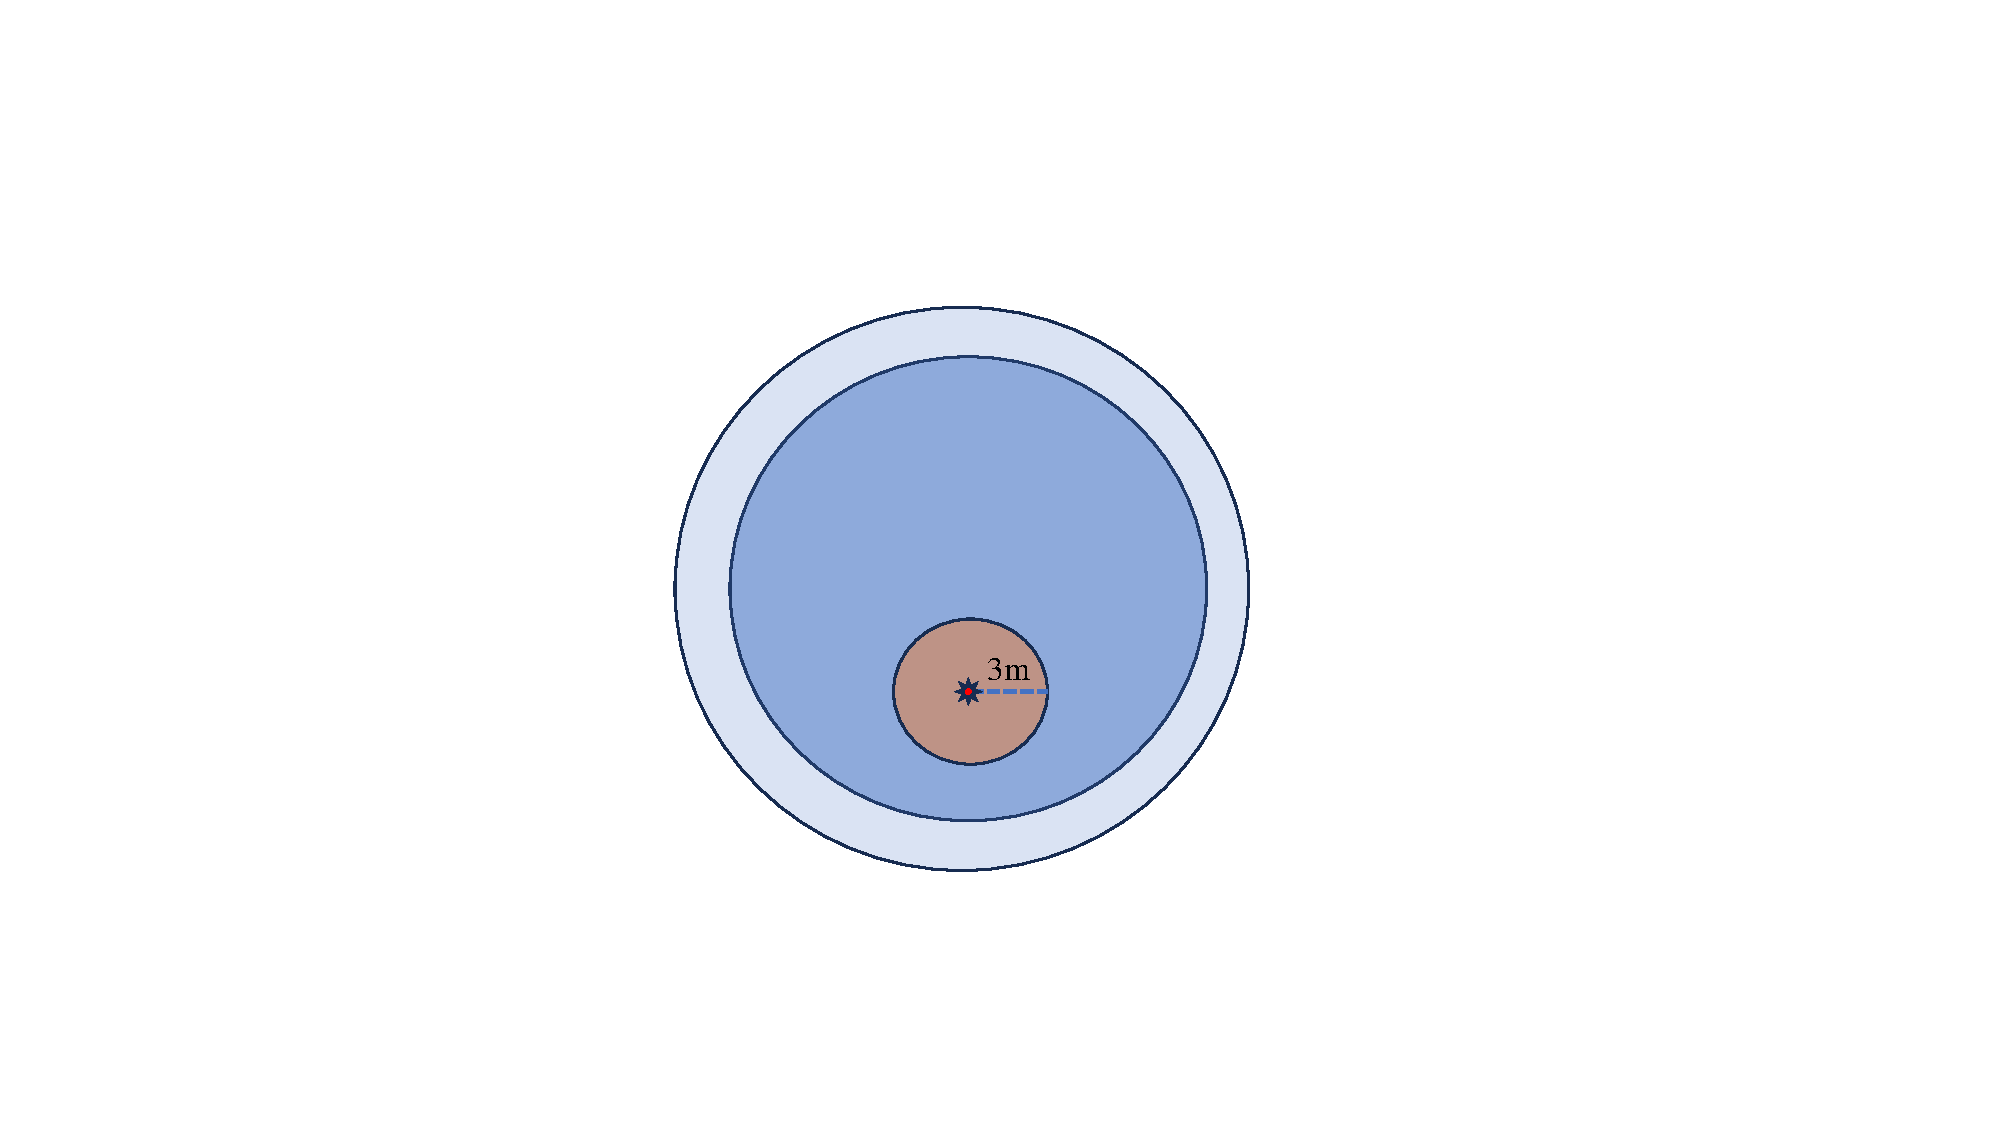
\includegraphics[width=0.5\textwidth]{neutron_calib/prompt/rCut.pdf}
	\caption{3-meter radius cut around the calibration source position}
	\label{fig:RtoSource}
\end{figure}
To account for the influence of the background energy distribution, data collected under identical conditions but without a calibration source at the same location are used.
For Run~3671, the background spectrum is derived from Run~3663.
To mitigate the impact of differing data acquisition durations, the energy spectra are normalized to live time, allowing event rates to serve as the primary comparison metric.
As shown in Fig.~\ref{fig:3671n20}, substantial background contamination remains in the energy spectrum despite the application of selection cuts.
After background subtraction, the $n_{20}$ distribution for \SI{4.4}{MeV} Gamma events is obtained. Similarly, for Run~3286, which utilizes an \ce{AmC} source, the background spectrum is derived from Run~3281. The $n_{20}$ distribution for \SI{6.1}{MeV} Gamma events is shown in Fig.~\ref{fig:3286n20}.
\begin{figure}[htbp]
	\centering
	\begin{subfigure}{0.5\textwidth}
		\centering
		\includegraphics[page=4,width=0.9\textwidth]{neutron_calib/prompt/3671.pdf}
		\caption{}
		\label{fig:3671n20}
	\end{subfigure}% 
	\begin{subfigure}{0.5\textwidth}
		\centering
		\includegraphics[page=4,width=0.9\textwidth]{neutron_calib/prompt/3286.pdf}
		\caption{}
		\label{fig:3286n20}
	\end{subfigure}
	\caption{The energy distribution of prompt signals. The black line represents the background energy distribution, the blue line represents the energy distribution of prompt signals, and the red line represents the prompt signal energy distribution after subtracting the background. \subref{fig:3671n20} is the result of Run~3671, representing the energy distribution of \SI{4.4}{MeV} Gamma. \subref{fig:3286n20} is the result of Run~3286, representing the energy distribution of \SI{6.1}{MeV} Gamma.}
	\label{fig:n20}
\end{figure}


\subsection{The search for delayed signals}
\subsubsection{The reconstruction of delayed signals}
\label{sec:coincidentRecon}
After applying the aforementioned selection criteria, prompt signal candidates are identified.
We then investigate the delayed signals arising from neutron capture events.
To reconstruct these delayed signals while reducing data volume, a coincidence reconstruction algorithm is employed.
As shown in Fig.~\ref{fig:delayedCoincidence}, a \SI{1000}{u\second} time window is used for delayed signal reconstruction.
For the study of accidental coincidence backgrounds, additional events are reconstructed within the 1000--\SI{2000}{u\second} interval.
\begin{figure}[htbp]
	\centering
	{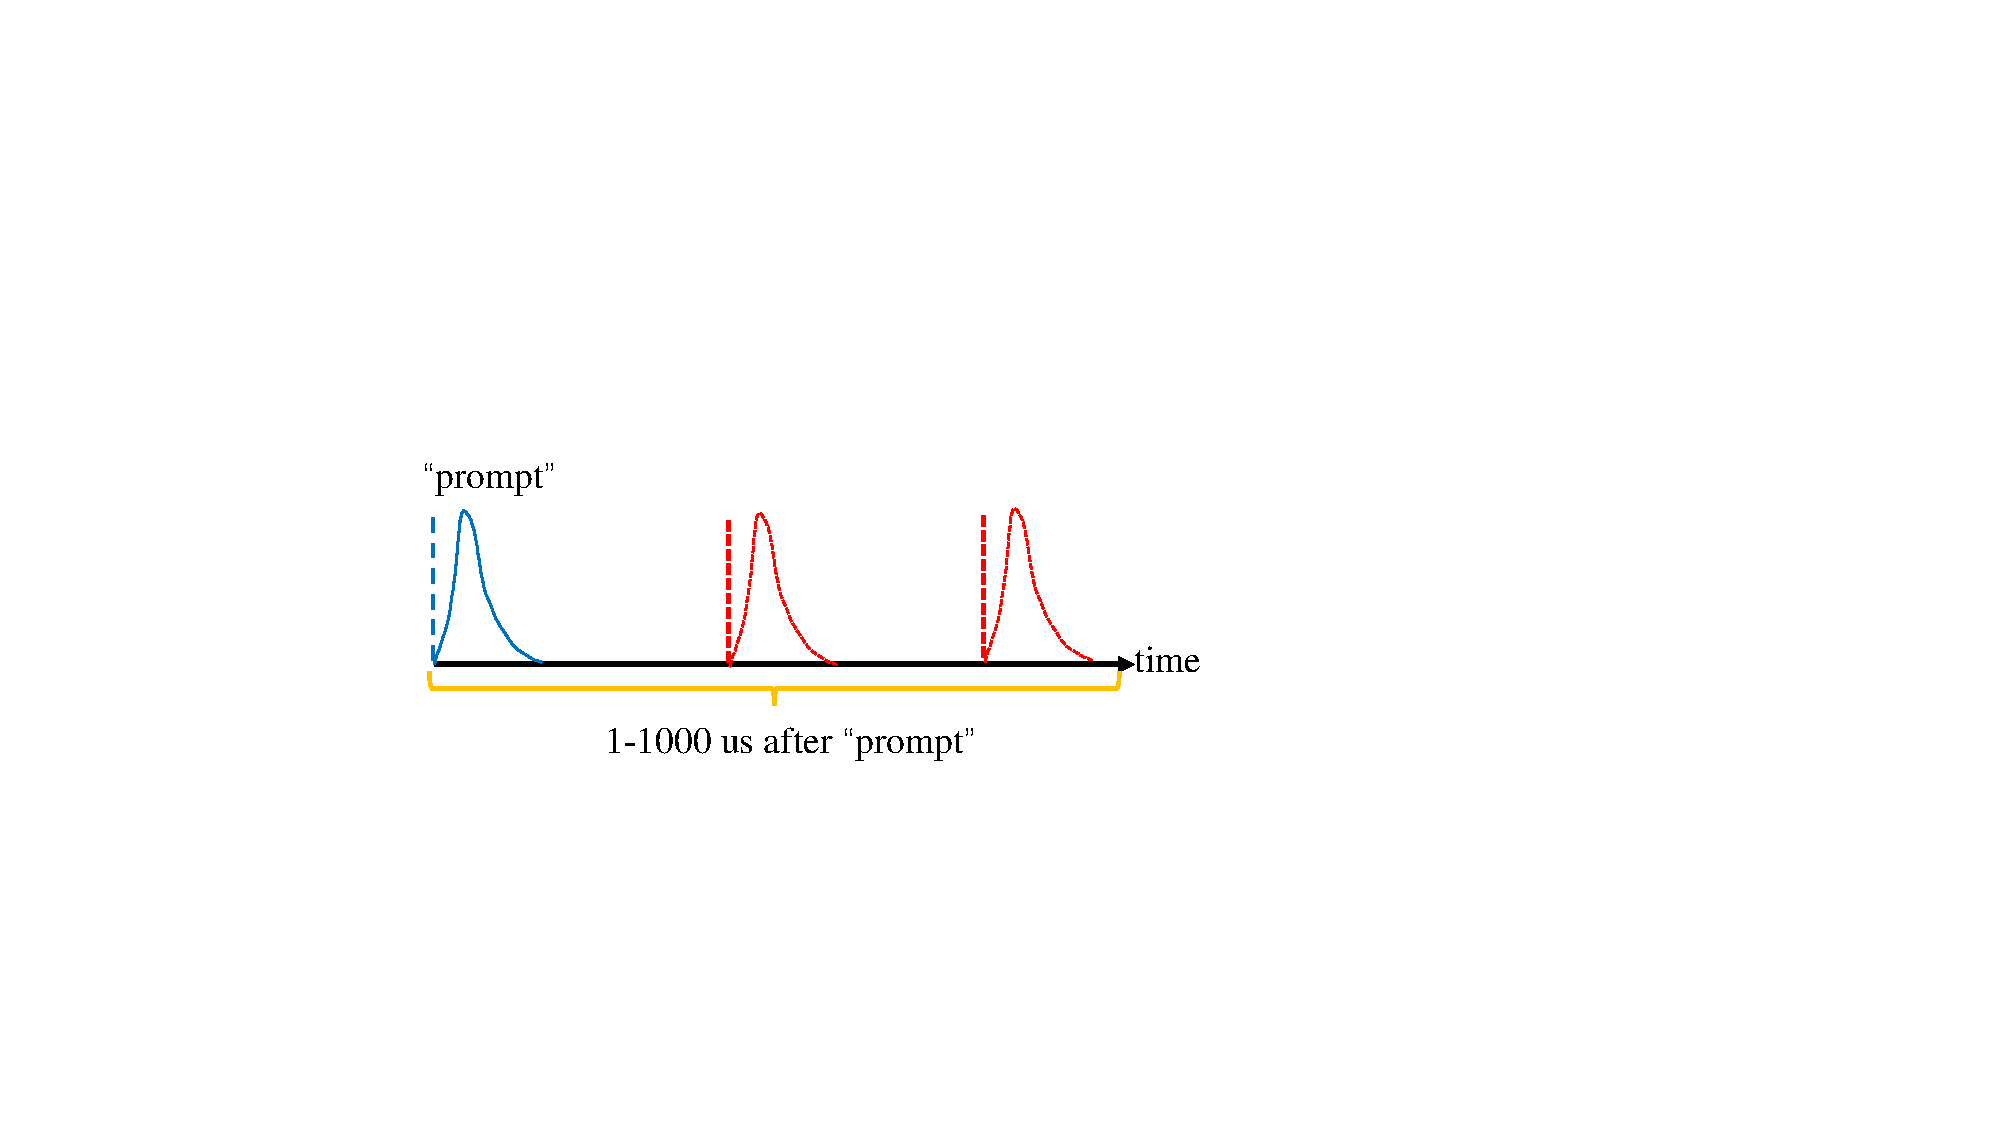
\includegraphics[width=0.5\textwidth]{neutron_calib/delayArea.pdf}}
	\caption{The delayed signal reconstruction time window.}
	\label{fig:delayedCoincidence}
\end{figure}
\subsubsection{The search for delayed signals}
\label{sec:nhSearch}
After the delayed signal reconstruction, we apply the following criteria to select delayed signals:
\begin{itemize}
	\item {The selection of prompt signals:
	      \begin{itemize}
		      \item Energy related cut: $n_{10}-n_{b}>15$.
		      \item Directional cut: $p_z/p>-0.8$.
		      \item Distance to the source: <\SI{3}{m}.
		      \item Muon veto: >\SI{500}{us}.
		      \item Background cut: $\delta A<-50$, $LE<40$.
	      \end{itemize}}
	\item {The selection of delayed signals:
	      \begin{itemize}
		      \item Energy related cut: $32<n_{20}-n_{b}<70$.
		      \item Coincident distance $dR<\SI{6}{m}$.
		      \item Directional cut: $p_z/p>-0.8$.
		      \item muon veto: >\SI{500}{us}.
		      \item Coincident time: $dT<\SI{1000}{us}$.
		      \item Background cut: $\delta A<-50$, $LE<40$.
	      \end{itemize}}
\end{itemize}
Following the series of selection procedures, an exponential fit,
\begin{equation}
	f(t)=A\exp(-t/\tau)+c
\end{equation}
is performed on the coincidence time distribution between prompt and delayed signals, as shown in Fig.~\ref{fig:delayFit}.
The extracted neutron capture lifetime is $203 \pm \SI{24}{u\second}$, in agreement with theoretical expectations within experimental uncertainties.
In parallel, the position distributions of both prompt and delayed signals are examined. As illustrated in Fig.~\ref{fig:coincidentPos}, events are strongly clustered around the calibration source location, consistent with the deployment geometry. These results demonstrate that the JUNO detector exhibits robust neutron detection capability during the water phase.


\begin{figure}[htbp]
	\centering
	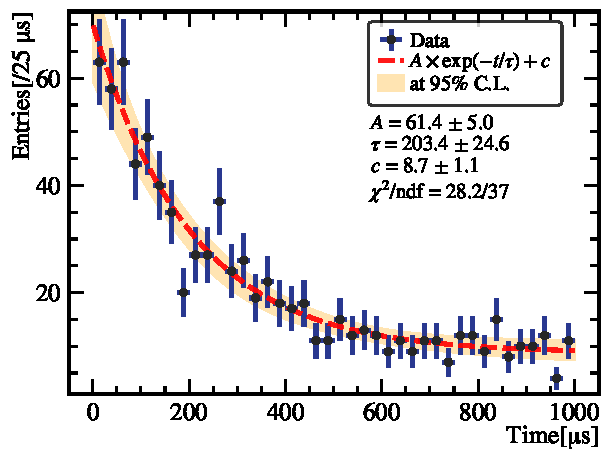
\includegraphics[width=0.5\textwidth]{neutron_calib/delayed/example/3671_dt.pdf}
	\caption{The coincident time fit.}
	\label{fig:delayFit}
\end{figure}

\begin{figure}[htbp]
	\centering
	\begin{subfigure}{0.5\textwidth}
		\centering
		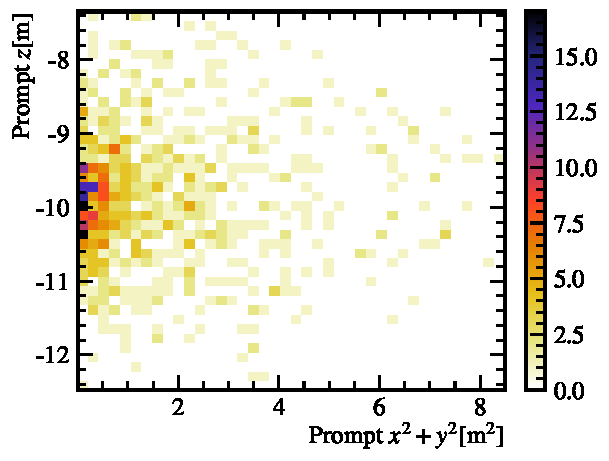
\includegraphics[width=0.9\textwidth]{neutron_calib/delayed/example/3671_coin_prompt_pos.pdf}
		\caption{}
		\label{fig:promptpos}
	\end{subfigure}%
	\begin{subfigure}{0.5\textwidth}
		\centering
		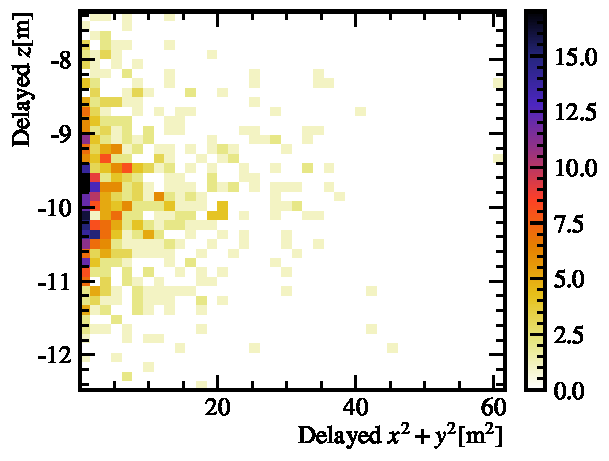
\includegraphics[width=0.9\textwidth]{neutron_calib/delayed/example/3671_coin_delayed_pos.pdf}
		\caption{}
		\label{fig:delayedpos}
	\end{subfigure}
	\caption{The position distribution of prompt and delayed signals.  \subref{fig:promptpos} is the position distribution of prompt signals, and \subref{fig:delayedpos} is the position distribution of delayed signals.}
	\label{fig:coincidentPos}
\end{figure}

\subsection{The low-energy threshold in water phase}
\label{subsec:low_energy}
Through a detailed analysis of calibration source data, distinct Gamma signals at \SI{6.1}{\MeV} and \SI{4.4}{\MeV} are identified, in addition to the characteristic \SI{2.2}{\MeV} Gamma signal originating from neutron capture on hydrogen.
To obtain a cleaner prompt signal energy spectrum, additional selection criteria are applied beyond the initial cuts.
Specifically, prompt events are required to satisfy $\delta A < -50$, and, for the \ce{AmC} source, the condition $n_{10} - n_{b} > 20$ is imposed.
These requirements enhance the purity of the prompt signal spectrum.
The energy spectrum of the \SI{4.4}{\MeV} Gamma is shown in Fig.~\ref{fig:promptene4}, while that of the \SI{6.1}{\MeV} Gamma is shown in Fig.~\ref{fig:promptene6}.
Furthermore, the energy cut used in the coincidence analysis is removed.
Coincidences occurring within \SI{1000}{u\second} are designated as signal, while those in the 1000--\SI{2000}{u\second} window are taken as background.
Using this approach, the energy distribution of the \SI{2.2}{\MeV} Gamma from neutron capture on hydrogen is obtained, as shown in Fig.~\ref{fig:promptene2}.

\begin{figure}[htbp]
	\centering
	\begin{subfigure}{0.5\textwidth}
		\centering
		\includegraphics[page=2,width=0.9\textwidth]{neutron_calib/light_yield.pdf}
		\caption{\SI{4.4}{MeV} Gamma signals}
		\label{fig:promptene4}
	\end{subfigure}%
	\hfill
	\begin{subfigure}{0.5\textwidth}
		\centering
		\includegraphics[page=3,width=0.9\textwidth]{neutron_calib/light_yield.pdf}
		\caption{\SI{6.1}{MeV} Gamma signals}
		\label{fig:promptene6}
	\end{subfigure}%

	\begin{subfigure}{0.5\textwidth}
		\centering
		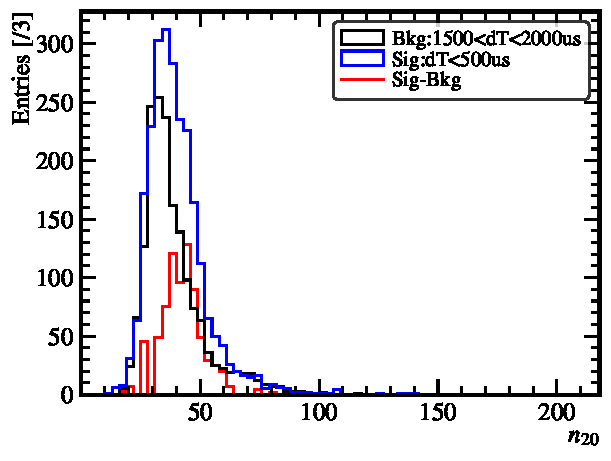
\includegraphics[page=1,width=0.9\textwidth]{neutron_calib/light_yield.pdf}
		\caption{\SI{2.2}{MeV} Gamma signals}
		\label{fig:promptene2}
	\end{subfigure}%
	\hfill
	\begin{subfigure}{0.5\textwidth}
		\centering
		\includegraphics[page=4,width=0.9\textwidth]{neutron_calib/light_yield.pdf}
		\caption{all selected Gamma signals}
		\label{fig:prompteneall}
	\end{subfigure}
	\caption{
		The $n_{20}$ distributions for \SI{2.2}{MeV}, \SI{4.4}{MeV}, and \SI{6.1}{MeV} Gamma signals, as well as the combined spectrum of all selected Gamma events.
	}
	\label{fig:energySpectrum46}
\end{figure}
After obtaining the energy spectra of the three characteristic signals, we perform Gaussian fitting to quantify their spectral parameters, as shown in Fig.~\ref{fig:FitYield}. When we use $n_{20}$ to estimate the energy, the light yield is $14.0\pm 0.1$~PE/MeV. Simultaneously, we estimate that each triggered physical event contains an average of \SI{8.1}{PE} originating from PMT dark noise and so on.
\begin{figure}[htbp]
	\centering
	\begin{subfigure}{0.5\textwidth}
		\centering
		\includegraphics[page=6,width=0.9\textwidth]{neutron_calib/light_yield.pdf}
		\caption{}
		\label{fig:fitene4}
	\end{subfigure}%
	\begin{subfigure}{0.5\textwidth}
		\centering
		\includegraphics[page=7,width=0.9\textwidth]{neutron_calib/light_yield.pdf}
		\caption{}
		\label{fig:fitene6}
	\end{subfigure}
	\begin{subfigure}{0.5\textwidth}
		\centering
		\includegraphics[page=5,width=0.9\textwidth]{neutron_calib/light_yield.pdf}
		\caption{}
		\label{fig:fitene2}
	\end{subfigure}%
	\begin{subfigure}{0.5\textwidth}
		\centering
		\includegraphics[page=8,width=0.9\textwidth]{neutron_calib/light_yield.pdf}
		\caption{}
		\label{fig:yield}
	\end{subfigure}
	\caption{Gaussian fit of the $n_{20}$ distribution of 4.4, 6.1 and \SI{2.2}{MeV} Gamma signals. \subref{fig:yield} is the Cherenkov light yiled fit.}
	\label{fig:FitYield}
\end{figure}

\section{The neutron capture detecting ability of JUNO in water phase}
\label{sec:tagEfficiency}
Neutron detection efficiency and SNR are critical parameters in the design and optimization of neutron detection systems, as it directly determines the accuracy and sensitivity of experimental measurements. In this section, we will discuss the neutron detection efficiency and SNR of the JUNO detector in the water.
In Sec.~\ref{sec:nhSearch}, the delayed signals were successfully reconstructed, and the neutron capture on hydrogen lifetime was obtained.
However, the efficiency of n-H capture tagging has yet to be determined.
To evaluate this, the prompt candidates are analyzed to calculate the n-H capture tagging efficiency.
After prompt signal reconstruction and selection, a total of $N_p$ prompt candidates are obtained, and the corresponding background contribution, $N_{pb}$, is estimated from dedicated background runs.
Among these prompt candidates, $N_{0}$ delayed candidates satisfy the n-H capture selection criteria.
Following a lifetime fit in which the coincidence time is binned into $N_b$ intervals, as illustrated in Fig.~\ref{fig:delayFit}, the number of accidental coincidence pairs is estimated as $c \times N_b$.
Thus, the net number of n-H capture events is calculated as $N_{\mathrm{nH}} = N_0 - c \times N_{b}$.
The tagging efficiency~($\eta$) and the signal-to-noise ratio~(SNR) are defined in Eq.~\eqref{eq:tagEfficiency}.
\begin{equation}
	\label{eq:tagEfficiency}
	\begin{aligned}
		 & \eta = (N_0 - c \cdot N_b) / (N_p - N_{pb})           \\
		 & \text{SNR} = (N_0 - c \cdot N_b) / \sqrt{c \cdot N_b}
	\end{aligned}
\end{equation}

As discussed in Sec.~\ref{sec:recon}, the application of background suppression techniques inevitably leads to a partial loss of delayed neutron capture events.
To evaluate the detector performance, a comprehensive parameter scan was conducted over an extended operational parameter space.
This systematic study aims to determine both the maximum attainable neutron detection efficiency and SNR for neutron tagging.
The parameters scanned for neutron tagging are summarized in Table~\ref{tab:param-scan}.
Following event selection, an n-H capture lifetime fit is performed.
The fitted lifetime is required to satisfy the following criteria:
\begin{itemize}
	\item Fitted lifetime falls within the range of 185--\SI{230}{us}. For calibration runs at $z=\SI{-16}{m}$: 3293 and 3342, the neutron capture lifetime constraint has been relaxed to the range of 170--\SI{250}{us}, while at $z=\SI{16}{m}$: 3279 and 3333, the constraint remains at 180--\SI{230}{us}, as evidenced in Fig.~\ref{fig:lifetime3671}.
	\item Contain the reference value of \SI{207}{us} within its $1\sigma$ uncertainty interval.
\end{itemize}

\begin{table}[htbp]
	\caption{Neutron Tagging Optimization Parameter Scan Specifications}%标题
	\label{tab:param-scan}
	\centering%把表居中
	\begin{tabular}{ccc}
		\toprule%第一道横线
		Parameters                   & Range      & Step or Point                                     \\
		\midrule%第二道横线 
		Coincident distance~($dR$,m) & 3--12      & 1                                                 \\
		Energy related~($n_{20}$)    & 0--49      & 2 when $9<n_{20}<25$; 1 when $25<n_{20}<50$       \\
		AIC criteria~($\delta A$)    & -70--0     & 5                                                 \\
		LE criteria~($LE$)           & 36--200    & 200, 150, 100, 50, 45, 43, 42, 41, 40, 39, 38 ,36 \\
		Goodness~($G_{vd}$)          & -0.1--0.15 & 0.02 when $G_{vd}<0$; 0.01 when $G_{vd}>0$        \\
		\bottomrule
	\end{tabular}
\end{table}
\begin{figure}[htbp]
	\centering
	\includegraphics[page=12,width=0.45\textwidth]{neutron_calib/delayed/coinsummary/3671.pdf}
	\caption{The fitted lifetime of Run~3671.}
	\label{fig:lifetime3671}
\end{figure}
Simultaneously, we examine the $\chi^2/ndf$ values of all fits, which consistently fall near 1.0, indicating excellent fit quality across the analyses, as shown in Fig.~\ref{fig:chi2}.
\begin{figure}[H]
	\centering
	\includegraphics[page=17,width=0.45\textwidth]{neutron_calib/delayed/coinsummary/3671.pdf}
	\caption{$\chi^2/ndf$ values changes with the $n_{20}$, but still around 1.0.}
	\label{fig:chi2}
\end{figure}

\subsection{The maximum neutron detection efficiency}
Maximizing neutron detection efficiency is crucial for capturing the largest possible fraction of neutron capture events, thereby improving statistical precision and extending the sensitivity of the detector to rare processes. In this context, the parameter scan results are examined to identify the configuration yielding the highest efficiency within the allowed lifetime selection criteria. As illustrated in Fig.~\ref{fig:High-eff}, the maximum neutron detection efficiency achieved is \SI{10}{\%} in Run~3671, with the corresponding selection parameters as shown in Table~\ref{tab:param-scan-eff}.

\begin{table}[htbp]
	\caption{\textbf{The parameters when get the highest efficiency}}%标题
	\label{tab:param-scan-eff}
	\centering%把表居中
	\begin{tabular}{ccc}
		\toprule%第一道横线
		Parameters                   & Selection     \\
		\midrule%第二道横线 
		Coincident distance~($dR$,m) & $<\SI{11}{m}$ \\
		Energy related~($n_{20}$)    & $>27$         \\
		AIC criteria~($\delta A$)    & $<-5$         \\
		LE criteria~($LE$)           & $<200$        \\
		Goodness~($G_{vd}$)          & $>0.02$       \\
		\bottomrule
	\end{tabular}
\end{table}

\begin{figure}[htbp]
	\centering
	\begin{subfigure}{0.5\textwidth}
		\centering
		\includegraphics[page=1,width=0.9\textwidth]{neutron_calib/delayed/coinsummary/3671.pdf}
		\caption{Efficiency vs. $dR$}
		\label{fig:effdR}
	\end{subfigure}%
	\begin{subfigure}{0.5\textwidth}
		\centering
		\includegraphics[page=2,width=0.9\textwidth]{neutron_calib/delayed/coinsummary/3671.pdf}
		\caption{Efficiency vs. $n_{20}$}
		\label{fig:effn20}
	\end{subfigure}
	\begin{subfigure}{0.5\textwidth}
		\centering
		\includegraphics[page=3,width=0.9\textwidth]{neutron_calib/delayed/coinsummary/3671.pdf}
		\caption{Efficiency vs. $\delta A$}
		\label{fig:effdA}
	\end{subfigure}%
	\begin{subfigure}{0.5\textwidth}
		\centering
		\includegraphics[page=4,width=0.9\textwidth]{neutron_calib/delayed/coinsummary/3671.pdf}
		\caption{Efficiency vs. $G_{vd}$}
		\label{fig:effGvd}
	\end{subfigure}
	\begin{subfigure}{0.5\textwidth}
		\centering
		\includegraphics[page=5,width=0.9\textwidth]{neutron_calib/delayed/coinsummary/3671.pdf}
		\caption{Efficiency vs. $LE$}
		\label{fig:effLE}
	\end{subfigure}
	\caption{Neutron detection efficiency as a function of five key selection parameters in Run~3671. The maximum efficiency achieved is \SI{11.7}{\%}.}
	\label{fig:High-eff}
\end{figure}

As shown in Fig.~\ref{fig:highestEffPos}, we select the highest-efficiency events in Run~3671.
The position distributions of the prompt and delayed signals are presented in Figs.~\ref{fig:3671HighestEffProPos} and \ref{fig:3671HighestEffDelPos}, respectively.
The prompt-signal distribution is consistent with the position of the deployed calibration source, while the delayed signals are observed to cluster around the corresponding prompt vertices.
This position correlation indicates that the delayed signals originate predominantly from neutron captures on hydrogen, as expected.
As illustrated in Fig.~\ref{fig:3671_HighestEffDtFit}, the fitted neutron-capture lifetime is measured to be $207.2 \pm \SI{47.2}{u\second}$, in agreement with the theoretical expectation.
The resulting fit yields a $\chi^{2}/\mathrm{ndf}$ of $27.3/30$, demonstrating good fit quality.

\begin{figure}[htbp]
	\begin{subfigure}{0.5\textwidth}
		\centering
		\includegraphics[page=5,width=0.9\textwidth]{neutron_calib/delayed/highesteff/3671.pdf}
		\caption{}
		\label{fig:3671HighestEffProPos}
	\end{subfigure}%
	\begin{subfigure}{0.5\textwidth}
		\centering
		\includegraphics[page=6,width=0.9\textwidth]{neutron_calib/delayed/highesteff/3671.pdf}
		\caption{}
		\label{fig:3671HighestEffDelPos}
	\end{subfigure}
	\caption{The position distribution when getting the highest efficiency in Run~3671. \subref{fig:3671HighestEffProPos} is the position distribution of the prompt signals, and \subref{fig:3671HighestEffDelPos} is of the delayed signals.}
	\label{fig:highestEffPos}
\end{figure}
\begin{figure}[H]
	\centering
	\includegraphics[page=3,width=0.45\textwidth]{neutron_calib/delayed/highesteff/3671.pdf}
	\caption{The lifetime fit when getting the highest efficiency events in Run~3671.}
	\label{fig:3671_HighestEffDtFit}
\end{figure}

As illustrated in Fig.~\ref{fig:SummaryEff}, neutron detection efficiency exceeding \SI{10}{\%} has been experimentally achieved, as validated through comprehensive calibration campaigns with \ce{AmBe} and \ce{AmC} neutron sources. During the calibrations on February 2-nd, the higher MM-trigger threshold resulted in an overall lower neutron detection efficiency compared to results of calibrations on February 2-nd. Simultaneously, significant asymmetry is observed between the positive and negative z-axis regions: detection efficiency in the negative z-axis is notably lower than in the positive z-axis, with the most pronounced deficit occurring at the \SI{16}{m} position. This demonstrates clear non-uniformity in JUNO's detector performance during the water phase.
\begin{figure}[htbp]
	\begin{subfigure}{0.5\textwidth}
		\centering
		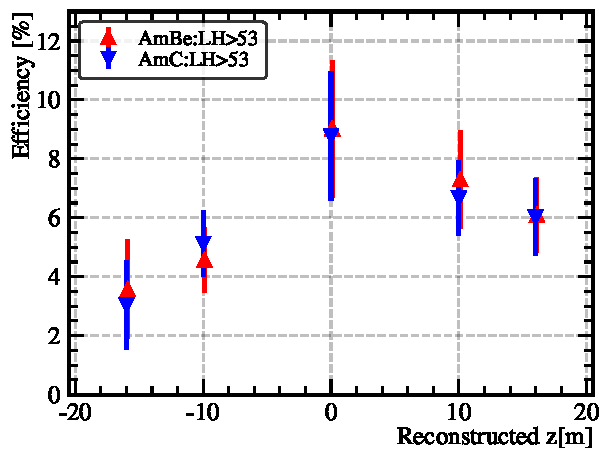
\includegraphics[width=0.9\textwidth]{neutron_calib/delayed/effsnr/0202_eff.pdf}
		\caption{}
		\label{fig:SummaryEff0202}
	\end{subfigure}%
	\begin{subfigure}{0.5\textwidth}
		\centering
		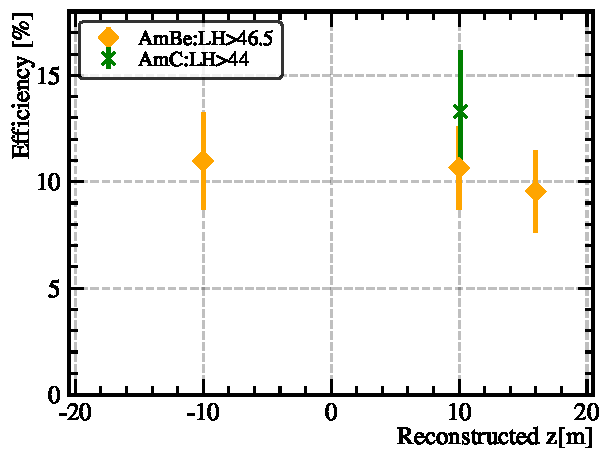
\includegraphics[width=0.9\textwidth]{neutron_calib/delayed/effsnr/0207_eff.pdf}
		\caption{}
		\label{fig:SummaryEff0207}
	\end{subfigure}
	\caption{The final highest neutron detection efficiency in all 14 calibration runs. \subref{fig:SummaryEff0202} is the result of calibrations on February 2-nd, and \subref{fig:SummaryEff0207} is of calibrations on February 7-th. }
	\label{fig:SummaryEff}
\end{figure}

\subsection{The highest neutron detection signal-to-noise ratio}
Maximizing SNR is essential for enhancing the clarity of true signal events relative to background fluctuations, thereby improving measurement accuracy and extending the detector's capability to resolve subtle physical effects. In this context, the parameter scan results are analyzed to identify the configuration yielding the highest SNR within the defined event selection criteria. As illustrated in Fig.~\ref{fig:High-snr}, the maximum SNR achieved is over 40 in Run~3671, with the corresponding selection parameters summarized in Table~\ref{tab:param-scan-snr}.

\begin{table}[htbp]
	\caption{\textbf{The parameters when get highest SNR}}%标题
	\label{tab:param-scan-snr}
	\centering%把表居中
	\begin{tabular}{ccc}
		\toprule%第一道横线
		Parameters                   & Selection    \\
		\midrule%第二道横线 
		Coincident distance~($dR$,m) & $<\SI{5}{m}$ \\
		Energy related~($n_{20}$)    & $>35$        \\
		AIC criteria~($\delta A$)    & $<-10$       \\
		LE criteria~($LE$)           & $<39$        \\
		Goodness~($G_{vd}$)          & $>0.12$      \\
		\bottomrule
	\end{tabular}
\end{table}

\begin{figure}[htbp]
	\centering
	\begin{subfigure}{0.5\textwidth}
		\centering
		\includegraphics[page=6,width=0.9\textwidth]{neutron_calib/delayed/coinsummary/3671.pdf}
		\caption{SNR vs. $dR$}
		\label{fig:snrdR}
	\end{subfigure}%
	\begin{subfigure}{0.5\textwidth}
		\centering
		\includegraphics[page=7,width=0.9\textwidth]{neutron_calib/delayed/coinsummary/3671.pdf}
		\caption{SNR vs. $n_{20}$}
		\label{fig:snrn20}
	\end{subfigure}
	\begin{subfigure}{0.5\textwidth}
		\centering
		\includegraphics[page=8,width=0.9\textwidth]{neutron_calib/delayed/coinsummary/3671.pdf}
		\caption{SNR vs. $\delta A$}
		\label{fig:snrdA}
	\end{subfigure}%
	\begin{subfigure}{0.5\textwidth}
		\centering
		\includegraphics[page=9,width=0.9\textwidth]{neutron_calib/delayed/coinsummary/3671.pdf}
		\caption{SNR vs. $G_{vd}$}
		\label{fig:snrGvd}
	\end{subfigure}
	\begin{subfigure}{0.5\textwidth}
		\centering
		\includegraphics[page=10,width=0.9\textwidth]{neutron_calib/delayed/coinsummary/3671.pdf}
		\caption{SNR vs. $LE$}
		\label{fig:snrLE}
	\end{subfigure}
	\caption{Neutron detection SNR as a function of five key selection parameters in Run~3671. The maximum SNR achieved is over 40.}
	\label{fig:High-snr}
\end{figure}

Similarly, as shown in Fig.~\ref{fig:highestSNRPos} and \ref{fig:3671_HighestSNRDtFit}, when operating at maximum SNR, the distributions of prompt and delayed signals remain consistent with expectations, and neutron capture lifetime fitting demonstrates excellent agreement with reference values.
\begin{figure}[htbp]
	\begin{subfigure}{0.5\textwidth}
		\centering
		\includegraphics[page=5,width=0.9\textwidth]{neutron_calib/delayed/highestsnr/3671.pdf}
		\caption{}
		\label{fig:3671HighestSNRProPos}
	\end{subfigure}%
	\begin{subfigure}{0.5\textwidth}
		\centering
		\includegraphics[page=6,width=0.9\textwidth]{neutron_calib/delayed/highestsnr/3671.pdf}
		\caption{}
		\label{fig:3671HighestSNRDelPos}
	\end{subfigure}
	\caption{The position distribution when getting the highest SNR in Run~3671. \subref{fig:3671HighestSNRProPos} is the position distribution of the prompt signals, and \subref{fig:3671HighestSNRDelPos} is of the delayed signals.}
	\label{fig:highestSNRPos}
\end{figure}
\begin{figure}[htbp]
	\centering
	\includegraphics[page=3,width=0.45\textwidth]{neutron_calib/delayed/highestsnr/3671.pdf}
	\caption{The lifetime fit when getting the highest SNR in Run~3671.}
	\label{fig:3671_HighestSNRDtFit}
\end{figure}

As shown in Fig.~\ref{fig:SummarySNR}, all 14 calibration runs demonstrate robust SNR performance. However, the calibrations on February 7-th exhibit significantly smaller statistical uncertainties due to higher neutron detection efficiency, resulting in substantially greater data volume for analysis.
\begin{figure}[htbp]
	\begin{subfigure}{0.5\textwidth}
		\centering
		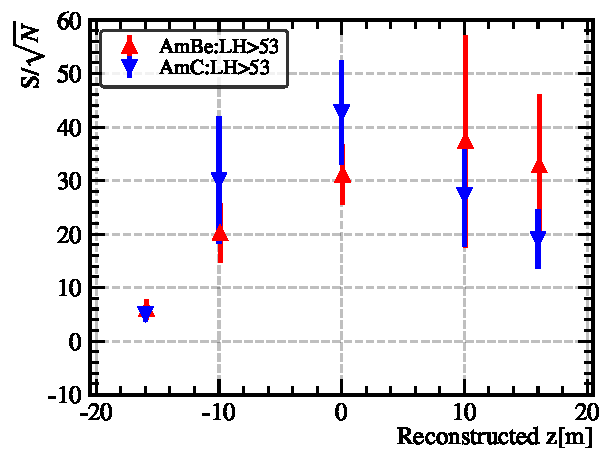
\includegraphics[width=0.9\textwidth]{neutron_calib/delayed/effsnr/0202_snr.pdf}
		\caption{}
		\label{fig:SummarySNR0202}
	\end{subfigure}%
	\begin{subfigure}{0.5\textwidth}
		\centering
		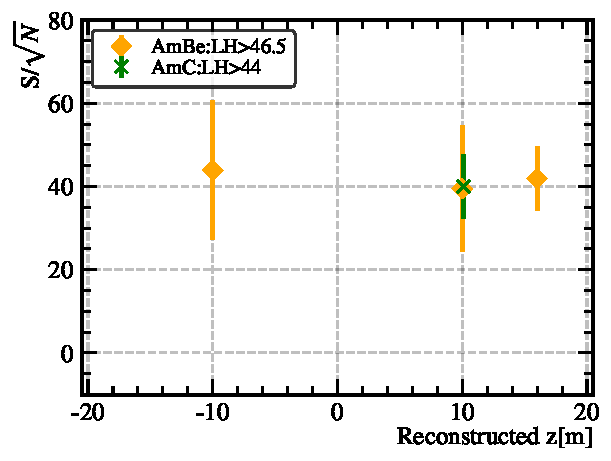
\includegraphics[width=0.9\textwidth]{neutron_calib/delayed/effsnr/0207_snr.pdf}
		\caption{}
		\label{fig:SummarySNR0207}
	\end{subfigure}
	\caption{The final highest neutron detection SNR in all 14 calibration runs. \subref{fig:SummarySNR0202} is the result of calibrations on February 2-nd, and \subref{fig:SummarySNR0207} is of calibrations on February 7-th. }
	\label{fig:SummarySNR}
\end{figure}


\subsection{The balance between neutron detection efficiency and SNR}
Based on these results, we observe the relationship between SNR and neutron detection efficiency, as shown in Fig.~\ref{fig:snr-efficiency}. The maximum achievable efficiency exceeds \SI{10}{\%}, while the SNR is lower than 20. This demonstrates a fundamental trade-off: stringent selection criteria yield excellent SNR at the cost of reduced efficiency, whereas relaxed cuts achieve high neutron detection efficiency but introduce significant background contamination.
\begin{figure}[htbp]
	\centering
	\includegraphics[page=21,width=0.5\textwidth]{neutron_calib/delayed/coinsummary/3671.pdf}
	\caption{The relationship between SNR and neutron detection efficiency. The maximum efficiency exceeds \SI{10}{\%}, and the maximum SNR surpasses 40.}
	\label{fig:snr-efficiency}
\end{figure}

\chapter{The measurement of spallation neutron yield in water phase}
From Sec.~\ref{sec:lowenergy}, we have demonstrated JUNO's neutron detection capability during its water phase. In the absence of calibration sources, this capability enables the detection of spallation neutrons produced by cosmic-ray muons traversing the detector. Because of the MM trigger threshold, we just use Run~3639~(around \SI{2}{h}) and 3677~(around \SI{5}{h}) for this measurement.
\section{The reconstruction of muon track}
Our muon reconstruction comes from Machine Learning~(JUNO-doc-13818), based on Global trigger data, around \SI{7}{h}.
To better characterize muon properties, we define the following parameters, as shown in Fig.~\ref{fig:muonTrackDef}.
\begin{itemize}
	\item $D_{tc}$: Distance from the CD center to the muon track
	\item $L_t$: Track length $L_t=2\times\sqrt{R^2_{CD}-D^2_{tc}}, R_{CD}=\SI{17.7}{m}$
	\item Distance from events to muon track: $dR$
\end{itemize}

From the distribution of $D_{tc}^2$ as shown in Fig.~\ref{fig:dfcc}, we observe cosmic-ray muons uniformly traversing the Central Detector. The Total PE distribution reveals that the majority of muons deposit between $10^5$ and $10^6$~\si{PE}, while a small fraction exhibit total PE counts below $10^5$, as evidenced in Fig.~\ref{fig:pe}. Fig.~\ref{fig:track-pe} demonstrates a strong correlation between muon track length and total PE for primary muons, forming a concentrated distribution band. However, events with $<10^5$~PE despite long reconstructed tracks likely originate from PMT flasher artifacts or electronic noise mimicking muon signals. Therefore, we implement a selection cut requiring muon candidates to have total PE $>10^5$. After the cut of $D_{tc}<\SI{17.7}{m}$ and Total PE $>10^5$, the muon event rate is \SI{4.03}{Hz}, which is consistent with the result of simulation~($0.004~\text{Hz/m}^2$)~\cite{muon207}. Also, the average energy of muon is \SI{207}{GeV}.
\begin{figure}[htbp]
	\centering
	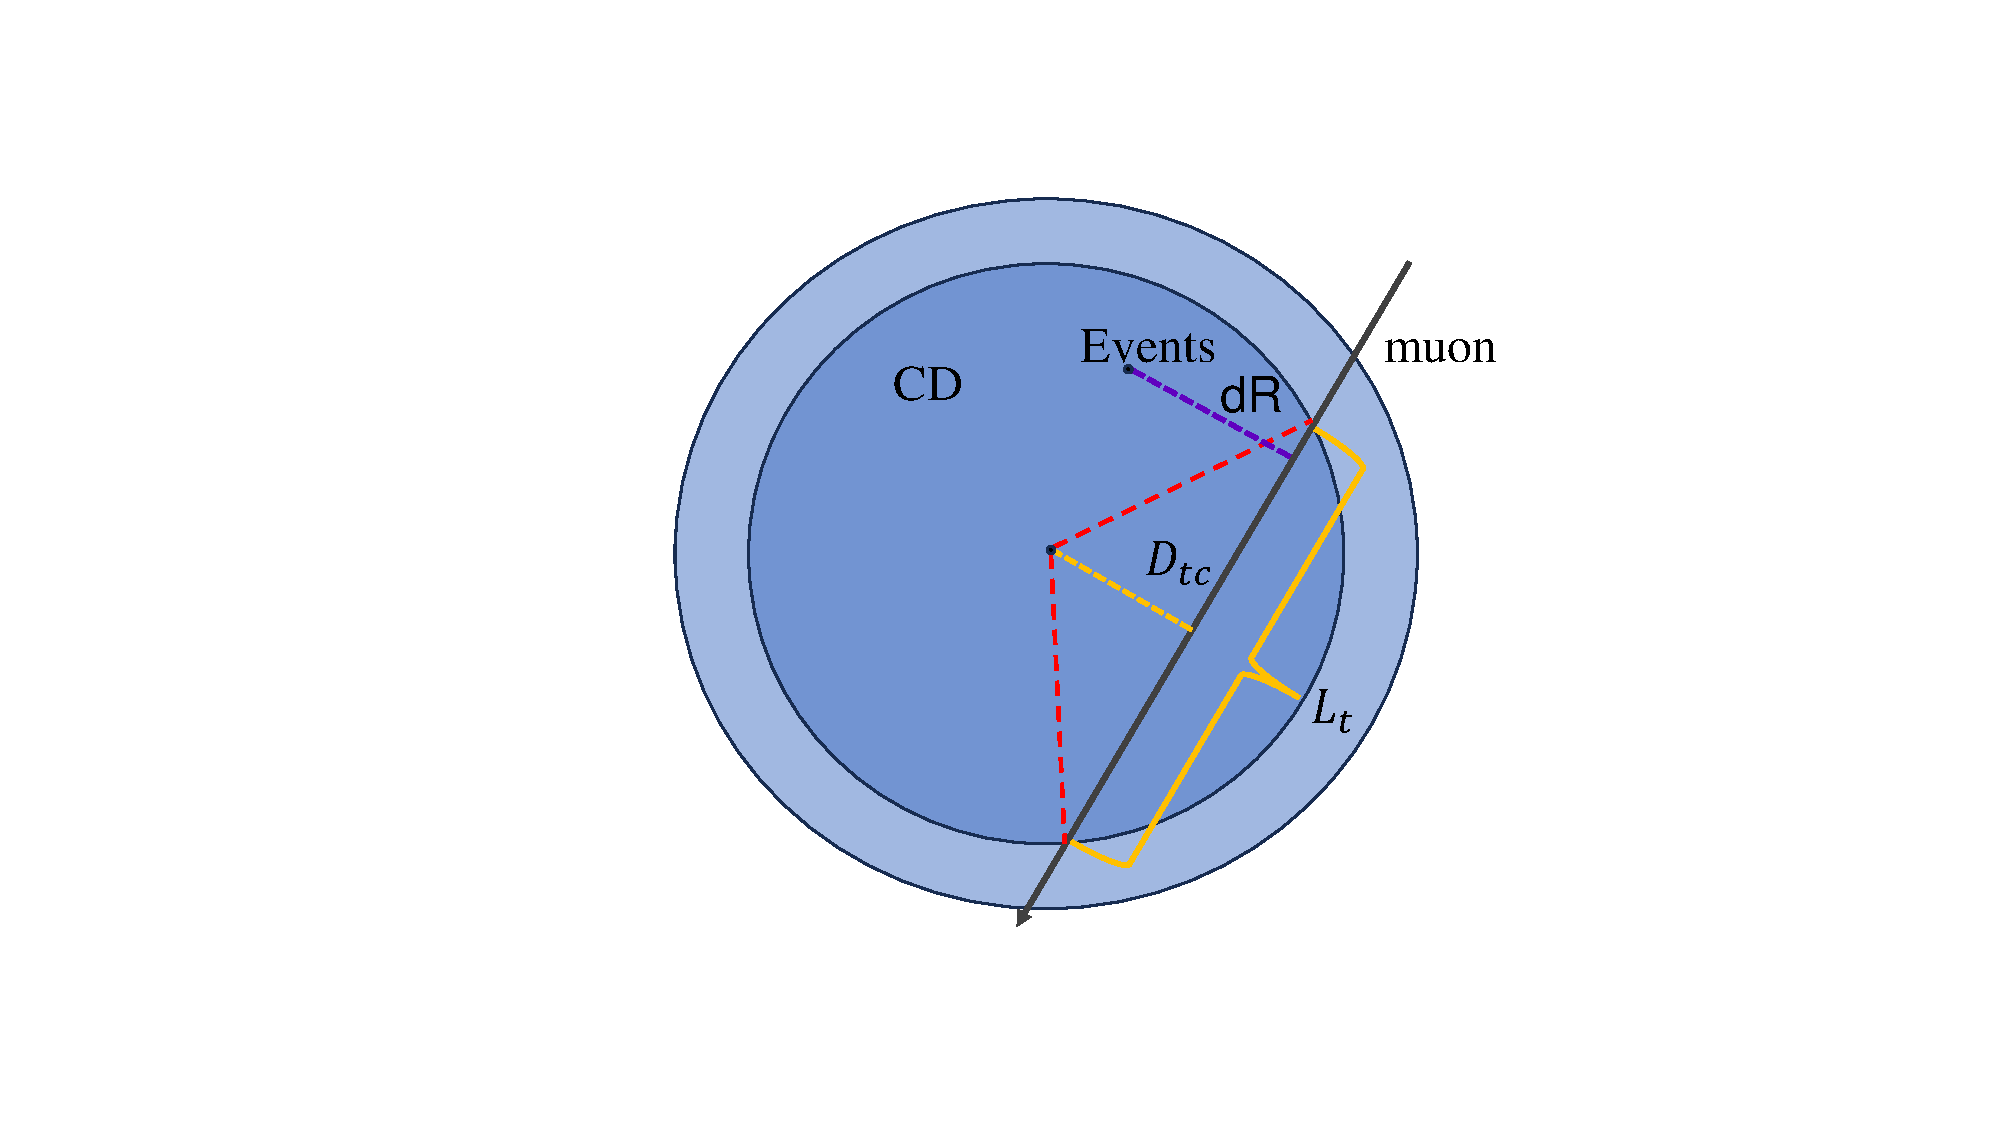
\includegraphics[width=0.5\textwidth]{spallation_n/track_define.pdf}
	\caption{The defination of parameters used in spallation neutron search.}
	\label{fig:muonTrackDef}
\end{figure}


\begin{figure}[htbp]
	\centering
	\begin{subfigure}{0.5\textwidth}
		\centering
		\includegraphics[page=4, width=0.9\textwidth]{spallation_n/yield_sdu.pdf}
		\caption{}
		\label{fig:dfcc}
	\end{subfigure}% 
	\begin{subfigure}{0.5\textwidth}
		\centering
		\includegraphics[page=6, width=0.9\textwidth]{spallation_n/yield_sdu.pdf}
		\caption{}
		\label{fig:pe}
	\end{subfigure}
	\begin{subfigure}{0.5\textwidth}
		\centering
		\includegraphics[page=7, width=0.9\textwidth]{spallation_n/yield_sdu.pdf}
		\caption{}
		\label{fig:track-pe}
	\end{subfigure}
	\caption{\subref{fig:dfcc} shows the distribution of $D_{tc}^2$, \subref{fig:pe} evidences the total PE of muons and \subref{fig:track-pe} demonstrates the relationship between total PE and the track length of muons.}
	\label{fig:MuonInfo}
\end{figure}

\section{The search for spallation neutron}
Similar to Sec.~\ref{sec:coincidentRecon}, we also use coincident reconstruction for spallation neutron, as shown in Fig.~\ref{fig:coinRecSPN}. For accidental coincident backgrounds, we reconstruct all events in 20--\SI{2000}{us} after muons. In 0--\SI{20}{us}, events are influenced by baseline, after-pulse and Michel electrons, and would not be included in our study.
\begin{figure}[htbp]
	\centering
	\includegraphics[width=0.5\textwidth]{spallation_n/spn_area.pdf}
	\caption{The coincident reconstruction of spallation neutrons}
	\label{fig:coinRecSPN}
\end{figure}

Validated through \ce{AmBe} and \ce{AmC} calibration, we get some basic cut for spallation neutrons:
\begin{itemize}
	\item Fiducial volume: $r<\SI{16}{m}$
	\item Background cut: $\delta A<-60$, $LE<50$, $G_{vd}>0.1$
	\item Energy related: $n_{20}<70$
\end{itemize}

After applying basical cuts, we observe residual downward events clustered near the detector center, as illustrated in Fig.~\ref{fig:pzcut}. To suppress this unknown background component, we implement an additional directional cut based on reconstructed direcition~$p_z/p>-0.75$.

\begin{figure}[htbp]
	\centering
	\includegraphics[page=16,width=0.45\textwidth]{spallation_n/yield_sdu.pdf}
	\caption{The distribution of $p_z/p$ in different regions}
	\label{fig:pzcut}
\end{figure}

For the coincident distance and energy cut, we choose the events in 50--\SI{650}{us} as signals and in 1400--\SI{2000}{us} as background.
After background subtraction, the distribution of $dR$ reveals significant event clustering within \SI{6}{m}, as evidenced in Fig.~\ref{fig:coinDisSPN}. This observation justifies implementing a position correlation cut of $dR<\SI{6}{m}$ to isolate true spallation neutron capture events. Similarly, in the $n_{20}$ distribution after background subtraction as shown in Fig.~\ref{fig:coinESPN}, we observe a prominent peak around \SI{35}{PE}. Using Gaussian fitting, the measured peak position is \SI{36.3}{PE}. This contrasts with the expected value of \SI{41}{PE} from that in calibration sources and the light-yield curve estimation of \SI{38.9}{PE}. The primary reason for this discrepancy lies in the calibration sources measuring light yield at fixed positions, whereas the current result represents the average PE expectation within \SI{16}{m} across the detector. Despite the numerical difference, these results remain consistent within the context of detector-scale estimation. Finally, we decide to use a cut of energy: $30<n_{20}<70$.
\begin{figure}[htbp]
	\centering
	\begin{subfigure}{0.5\textwidth}
		\centering
		\includegraphics[page=17, width=0.9\textwidth]{spallation_n/yield_sdu.pdf}
		\caption{}
		\label{fig:coinDisSPN0}
	\end{subfigure}% 
	\begin{subfigure}{0.5\textwidth}
		\centering
		\includegraphics[page=18, width=0.9\textwidth]{spallation_n/yield_sdu.pdf}
		\caption{}
		\label{fig:coinDisSPN1}
	\end{subfigure}
	\caption{The coincident distance distribution.}
	\label{fig:coinDisSPN}
\end{figure}

\begin{figure}[htbp]
	\centering
	\begin{subfigure}{0.5\textwidth}
		\centering
		\includegraphics[page=19, width=0.9\textwidth]{spallation_n/yield_sdu.pdf}
		\caption{}
		\label{fig:coinESPN0}
	\end{subfigure}% 
	\begin{subfigure}{0.5\textwidth}
		\centering
		\includegraphics[page=20, width=0.9\textwidth]{spallation_n/yield_sdu.pdf}
		\caption{}
		\label{fig:coinESPN1}
	\end{subfigure}
	\caption{The distribution of energy related parameter $n_{20}$}
	\label{fig:coinESPN}
\end{figure}

At this stage, we calculate the number of spallation neutrons using capture lifetime fitting in [30, \SI{930}{us}], as shown in Fig.~\ref{fig:lifeSPNSDU}. From the fit result, $987\pm 119$ spallation neutron events are selected. We similarly examine the position distribution of selected events. By using coincidences within the 1100--\SI{2000}{us} window as background and subtracting them. In both background and selected events, we observe event clustering at the detector center. After background subtraction, we obtain the position distribution of spallation neutrons. The position distribution in the upper hemisphere of the detector exceeds that in the lower hemisphere. This asymmetry aligns with the detector non-uniformity observed during calibration source studies.
\begin{figure}[htbp]
	\centering
	\includegraphics[page=8,width=0.5\textwidth]{spallation_n/yield_sdu.pdf}
	\caption{The lifetime fitting of spallation neutron.}
	\label{fig:lifeSPNSDU}
\end{figure}

\begin{figure}[htbp]
	\centering
	\begin{subfigure}{0.5\textwidth}
		\centering
		\includegraphics[page=9, width=0.9\textwidth]{spallation_n/yield_sdu.pdf}
		\caption{}
		\label{fig:coinPOS_sig}
	\end{subfigure}% 
	\begin{subfigure}{0.5\textwidth}
		\centering
		\includegraphics[page=10, width=0.9\textwidth]{spallation_n/yield_sdu.pdf}
		\caption{}
		\label{fig:coinPOS_bkg}
	\end{subfigure}
	\begin{subfigure}{0.5\textwidth}
		\centering
		\includegraphics[page=11, width=0.9\textwidth]{spallation_n/yield_sdu.pdf}
		\caption{}
		\label{fig:coinPOS_ex}
	\end{subfigure}
	\caption{The position distribution. \subref{fig:coinPOS_sig} evidences the distribution of the selected events. \subref{fig:coinPOS_sig} shows the distribution of the background events in 1100--\SI{2000}{us} after muon. \subref{fig:coinPOS_ex} displays the result of histogram subtraction between two distributions}
	\label{fig:coinPOS}
\end{figure}

\section{The spallation neutron yield calculation}
By combining data from the previous 14 calibration runs, we can estimate the average neutron detection efficiency within a 16-meter radius of the detector. We employed an $R^3$-weighted position averaging method to compute the position-dependent neutron detection efficiency, yielding a volume-averaged efficiency of $3.3\pm\SI{0.4}{\%}$, and the final efficiencies in our study are in Table.~\ref{tab:spn_eff}.
The spallation neutron yield $Y_n$ is defined as the neutron production rate per unit muon track length and per unit density, as defined in Eq.~\eqref{eq:yn}.
\begin{equation}
	\label{eq:yn}
	Y_n = \frac{N_n}{\rho N_{muon}L_{t,ave}}= \frac{N_n}{\rho \Sigma_{muon} L_t}
\end{equation}
Only consider the statistical uncertainty, the spallation neutron yield is $Y_n = (2.31\pm0.41 \text{(stat.)})\times 10^{-4} \mu^{-1}\text{g}^{-1}\text{cm}^2$.
\begin{table}[H]
	\caption{The efficiencies in spallation neutron search}%标题bottomrule
	\label{tab:spn_eff}
	\centering%把表居中
	\begin{tabular}{ccc}
		\toprule%第一道横线
		                       & Effieciency          \\
		\midrule%第二道横线 
		Neutron Tag            & $3.3\pm\SI{0.4}{\%}$ \\
		Fiducial volume        & \SI{73.9}{\%}        \\
		Coincident time window & \SI{85.4}{\%}        \\
		Direcition cut         & \SI{87.5}{\%}        \\
		\bottomrule
	\end{tabular}
\end{table}

Simultaneously, there are three primary sources of systematic uncertainty. The first kind comes from the muon track reconstruction. We found a systematic \SI{0.2}{\%} bias between reconstructed muon track lengths and their true values, as shown in Fig.~\ref{fig:muontrackUncerntainty}. Consequently, we attribute a \SI{0.2}{\%} systematic uncertainty to muon track reconstruction in our analyses.
The second source of systematic uncertainty originates from neutron count variations induced by coincident distance selection. We perform parameter scans across multiple coincidence distances, as evidenced in Fig.~\ref{fig:muonCountUncerntainty} and quantified the systematic uncertainty using the maximum deviation from the central value obtained at different coincident distances.
The final source of systematic uncertainty stems from detector inhomogeneity and discrepancies between simulation and experimental data. During \ce{AmBe} and \ce{AmC} calibrations, the neutron detection efficiency at $z = \SI{-16}{m}$ approaches zero, as shown in Fig.~\ref{fig:SPNsourceCalib}. To quantify the impact of this local efficiency anomaly on the global average efficiency, we perform a parameter scan across a $5\sigma$ range of efficiency uncertainty (0 to \SI{1.2}{\%}) based on the fitting results at this position. The range in the resulting detection efficiency is then adopted as the systematic uncertainty, as shown in Fig.~\ref{fig:muonEffUncerntainty}. All the systematic efficiencies are summarized in Table.~\ref{tab:spn_eff_un}. Our final result of spallation neutron yield measurement is $Y_n = (2.31\pm0.22\text{(sys.)}\pm0.41 \text{(stat.)}) \times 10^{-4}\mu^{-1}\text{g}^{-1}\text{cm}^2$. As shown in Fig.~\ref{fig:yield_final}, our measurements in the water phase demonstrate statistically significant consistency with Super-Kamiokande's benchmark results across key neutron detection parameters, validating the calibration methodology and detector performance.
\begin{figure}[htbp]
	\centering
	\includegraphics[width=0.5\textwidth]{spallation_n/muonTrack_err.pdf}
	\caption{The track length distribution of reconstructed muon and their truth.}
	\label{fig:muontrackUncerntainty}
\end{figure}

\begin{figure}[htbp]
	\centering
	\includegraphics[page=21, width=0.5\textwidth]{spallation_n/yield_sdu.pdf}
	\caption{We scan $dR$ from in 3--\SI{9}{m}, and calculate the number of neutrons.}
	\label{fig:muonCountUncerntainty}
\end{figure}

\begin{figure}[htbp]
	\centering
	\begin{subfigure}{0.5\textwidth}
		\centering
		\includegraphics[page=9,width=0.9\textwidth]{spallation_n/eff_err.pdf}
		\caption{}
		\label{fig:SPNsourceCalib}
	\end{subfigure}% 
	\begin{subfigure}{0.5\textwidth}
		\centering
		\includegraphics[page=11,width=0.9\textwidth]{spallation_n/eff_err.pdf}
		\caption{}
		\label{fig:muonEffUncerntainty}
	\end{subfigure}

	\caption{The estimation of uncertainty from efficiency. \subref{fig:SPNsourceCalib} evidences the efficiency estimated from \ce{AmBe} calibration with the same selection of spallation neutron. \subref{fig:muonEffUncerntainty} shows that the final efficiency is influenced by the efficiency at $z=\SI{-16}{m}$.}
	\label{fig:muonEffUncer}
\end{figure}

\begin{table}[htbp]
	\caption{The systematic uncertainty in spallation neutron search}%标题
	\label{tab:spn_eff_un}
	\centering%把表居中
	\begin{tabular}{ccc}
		\toprule%第一道横线
		                              & uncertainty       \\
		\midrule%第二道横线 
		Muon track reconstruction     & \SI{0.2}{\%}      \\
		Number of spallation neutrons & $\pm92$           \\
		The detection efficiency      & $\pm\SI{0.3}{\%}$ \\
		\bottomrule
	\end{tabular}
\end{table}

\begin{figure}[htbp]
	\centering
	\includegraphics[page=22,width=0.45\textwidth]{spallation_n/yield_sdu.pdf}
	\caption{The final yield measurement. The result of SK comes from~\cite{SK_spnYn}, of SNO comes from~\cite{sno_spnYn} and the prediction of LS is from \cite{Predict_LS_Wang}.}
	\label{fig:yield_final}
\end{figure}
\subsection{Cross check using water-pool reconstructed muon}
In order to cross-check the muon reconstruction in the water phase, we repeat the analysis using the water pool muon reconstruction method~(JUNO-doc-13604). Except for the removal of the muon selection cut, all other selection criteria remain identical to those applied when using CD muons. The final result is $Y_n =( 2.32\pm0.19\text{(sys.)}\pm0.44 \text{(stat.)}) \times 10^{-4}\mu^{-1}\text{g}^{-1}\text{cm}^2$, as shown in Fig.~\ref{fig:yield_sjtu_yield} and \ref{fig:yield_sjtu22}. Those two results are consistent with each other.

\begin{figure}[htbp]
	\centering
	\begin{subfigure}{0.5\textwidth}
		\centering
		\includegraphics[page=8, width=0.9\textwidth]{spallation_n/yield_sjtu.pdf}
		\caption{}
		\label{fig:yield_sjtu8}
	\end{subfigure}%
	\begin{subfigure}{0.5\textwidth}
		\centering
		\includegraphics[page=11, width=0.9\textwidth]{spallation_n/yield_sjtu.pdf}
		\caption{}
		\label{fig:yield_sjtu11}
	\end{subfigure}
	\begin{subfigure}{0.5\textwidth}
		\centering
		\includegraphics[page=22, width=0.9\textwidth]{spallation_n/yield_sjtu.pdf}
		\caption{}
		\label{fig:yield_sjtu22}
	\end{subfigure}
	\caption{\subref{fig:yield_sjtu8} is the lifetime fitting of spallation neutrons using WP muons. \subref{fig:yield_sjtu11} is the position distribution after extracting background. \subref{fig:yield_sjtu22} is the yield of spallation neutron using WP muons.}
	\label{fig:yield_sjtu_yield}
\end{figure}

\subsection{The prediction of $Y_n$ in water}
At present, regarding the research on the muon-induced spallation neutron yield, multiple underground experiments have completed the measurements. Among them, most experiments measured the yield in LS. SK~\cite{SK_spnYn} was the first to complete the measurement of the yield in the water phase, and SNO~\cite{sno_spnYn} experiment completed the measurement of the yield in heavy water. The relevant results are summarized in Tab.~\ref{tab:syn_summary}.

\begin{table}[htbp]
	\centering
	\caption{The measurement of spallation neutron yield}
	\label{tab:syn_summary}
	\begin{tabular}{cccc}
		\toprule
		Target          & Experiment                            & $E_{\mu}$ (\si{GeV}) & $Y_n$ ($\mu^{-1}\mathrm{g}^{-1}\mathrm{cm}^{2}$) \\
		\midrule
		LS              & Hertenberger~\cite{spnYn_hertenberge} & 13                   & $(2.0 \pm 0.7) \times 10^{-5}$                   \\
		LS              & Boehm~\cite{spnYn_Boehm}              & 16.5                 & $(3.6 \pm 0.4) \times 10^{-5}$                   \\
		LS              & DayaBayEH2~\cite{spnYn_Daya_bay}      & $64.7\pm3.9$         & $(10.22 \pm 0.87) \times 10^{-5}$                \\
		LS              & Aberdeen~\cite{spnYn_Aberdeen}        & $89.8\pm2.9$         & $(1.19 \pm 0.29) \times 10^{-4}$                 \\
		LS              & DayaBayEH3~\cite{spnYn_Daya_bay}      & $143.0\pm8.6$        & $(1.703 \pm0.122) \times 10^{-4}$                \\
		LS              & KamLAND~\cite{spnYn_KamLAND}          & $268\pm8$            & $(2.8 \pm 0.3) \times 10^{-4}$                   \\
		LS              & Borexino~\cite{spnYn_Borexino}        & $280$                & $(3.10 \pm 0.11) \times 10^{-4}$                 \\
		LS              & JNE~\cite{spnYn_JNE}                  & $\sim 360$           & $(3.37 \pm 1.44) \times 10^{-4}$                 \\
		Water~(\ce{Gd}) & SK~\cite{SK_spnYn}                    & $259\pm9$            & $(2.76 \pm 0.26) \times 10^{-4}$                 \\
		Water           & This work                             & $207$                & $(2.31 \pm 0.45) \times 10^{-4}$                 \\
		Hevey Water     & SNO~\cite{sno_spnYn}                  & $363\pm1.2$          & $(7.28 \pm 1.59) \times 10^{-4}$                 \\
		% 请在此处添加其他行数据
		\bottomrule
	\end{tabular}
\end{table}

In LS, the yield of spallation neutrons is positively correlated with the average energy of muons and can be described by an empirical formula, as shown in Eq.~\eqref{eq:yn_formular}~\cite{spnYn_Boehm,Predict_LS_Wang,Formuler_1,Predict_LS_Mei}. Wang, Y.-F. et al~\cite{Predict_LS_Wang} and Mei. et al~\cite{Predict_LS_Mei} , Kudryavtsev. et al~\cite{Kudryavtsev} and Daya Bay\cite{spnYn_Daya_bay} used some yield measurement to fit and their fit results are in Tab.~\ref{tab:fit_E_mu}.
\begin{equation}
	\label{eq:yn_formular}
	Y_n(E_{\mu}) = a_{\mu}E_{\mu}^{b_{\mu}}
\end{equation}

\begin{table}[htbp]
	\centering
	\caption{The fitted parameters of Eq.~\eqref{eq:yn_formular}}
	\label{tab:fit_E_mu}
	\begin{tabular}{cccc}
		\toprule
		                 & Fitted $a_{\mu}$($10^{-6}\mu^{-1}\mathrm{g}^{-1}\mathrm{cm}^{2}$) & Fitted $b_{\mu}$ \\
		\midrule
		Wang Y.-F. et al & 4.14                                                              & 0.74             \\
		Mei. et al       & 3.824                                                             & 0.849            \\
		Kudryavtsev      & 3.2                                                               & 0.79             \\
		Daya Bay         & 4.0                                                               & 0.77             \\
		This work        & 3.36                                                              & 0.793            \\
		% 请在此处添加其他行数据
		\bottomrule
	\end{tabular}
\end{table}

As shown in Fig.~\ref{fig:yield_fit_formuler}, with the exception that the fitting results of Mei et al. deviate notably from these experiments, the other three fitting results are generally in agreement with the experimental measurements, despite some minor discrepancies. Meanwhile, the three prediction results incorporate the results of the two measurements in water phase. This indicates that the predicted curve of the neutron yield of LS as a function of the average muon energy can approximately characterize the neutron yield of the water phase. Additionally, calculations were performed based on the two measurement results from the water phase of JUNO and SK, and the result is $a_{\mu}=3.36\times10^{-6}\mu^{-1}\mathrm{g}^{-1}\mathrm{cm}^{2}$, $b_{\mu}=0.793$.

\begin{figure}[htbp]
	\centering
	\includegraphics[page=23,width=0.6\textwidth]{spallation_n/yield_sdu.pdf}
	\caption{The inverted triangle markers denote the measurements outcome in LS, the square markers represent the measurement results in heavy water, and the circular markers indicate the measurement findings in water. The dashed line depicts the yield curve derived from fitting the measurement results in LS, while the red solid line represents the yield prediction curve computed using the measurement results in the water phase. }
	\label{fig:yield_fit_formuler}
\end{figure}